%
% A Real Chapter
\chapter{Background}

% Modeling of Walking
\section{Modeling of Walking}

\subsection{Simple Walking Model}
Mass, inertia, finite-sized foot.
\subsection{Linear Inverted Pendulum Model}
In modeling of walking, one of the most important assumptions often made is the modeling of the stance leg as a \acf{LIP}, as for example in \cite{kajita20013d}. Besides this, a not-linearized inverted pendulum is also widely used in the modeling of walking \cite{kuo2005energetic}. For planning and control however, a linearized description is desirable. In the \ac{2D} \ac{LIP} equations of motion
\begin{equation}
\ddot{x}=\frac{g}{l}x
\label{eq:LIPeom}
\end{equation}
where $l$ is the pendulum length and $x$ the Cartesian x-coordinate of the pendulum tip, the motion of the tip along the x-axis does not affect $l$. At any position $x$, a local virtual straight pendulum can be considered, so this motion is at a constant height and $l=z_0$  holds. As in \ac{3D} by the linear model the system dynamics can be decoupled, the dynamics in $y$-direction read the same: $\ddot{y}=\frac{g}{l} y$. In \figref{fig:3dlip} this motion is visualized if the \ac{CoM} is relatively far from from the base. The pendulum base lies in the origin and $\boldsymbol{x} = [x,y]^T$ is the \ac{2D} \ac{CoM} projection on the horizontal plane. Because the \ac{LIP} assumption holds, the vertical component of the leg force $\boldsymbol{f}$ has to cancel out gravity acceleration: $f_z=mg$.
\begin{figure}[h]
\centering
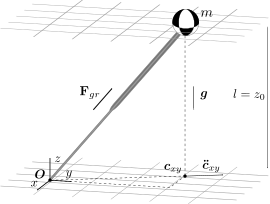
\includegraphics[width=0.5\textwidth]{STYLESTUFF/3DCoMwithoutfoot.png}
\caption{\ac{3D} motion of \ac{LIP} model.}
\label{fig:3dlip}
\end{figure}
\subsection{Height Varying Models}
Models that are related to the \ac{LIP} model, but consider height variations are to be destinguished in two types: the inverted pendulum model, and a model with varying pendulum length. The inverted pendulum model is in human motion studies often used, as for example in \cite{kuo2005energetic}. The model with varying pendulum lenght is the most generic models of all mentioned. Considering all models in \ac{2D} with point-foot, with the \ac{LIP} model and the inverted pendulum model the trajectories are known in advance. With the varying leg length model, an infinite amount of trajectories is theoretically possible to bring the pendulum tip from one point to the other.
% Ground Reference Points
\section{Measured Quantities \& Ground Reference Points in Walking}

\subsection{Ground Reaction Force}
A common approach for quantifying the dynamics of a walker, either a human or a robot, is the use of a \ac{GRF}, coming a from a single point of application on the ground. The magnitude and direction of the force vector, the gravitational vector, other external forces and the robots state determine the dynamics of the system. 


\subsection{The \ac{CoP}}
The feet attached to the \ac{LIP} robot model increase the possibilities to control its motion. The ankles can apply a torque that would virtually move the position of the base of the inverted pendulum, so that the linear acceleration on the \ac{CoM} as in Eq. \eqref{eq:LIPeom} and the capture point as in Eq. \eqref{eq:cp} change. The new virtual base is called the \ac{CoP}. By its definition, this point only lives within the support polygon \cite{vukobratovic2004zero}. In \figref{fig:3dlipfoot} the definition of the \ac{CoP} is visualized. If the point mass is restricted to move on a constant height, the vertical component of $\boldsymbol{f'}$ counteracts gravity: $f'_z=g$. 
\begin{figure}[h]
\centering
\includegraphics[width=0.5\textwidth]{STYLESTUFF/3DCoMwithfoot.png}
\caption{\ac{3D} motion of \ac{LIP} model with foot. The yellow cross points out the \ac{CoP} location.}
\label{fig:3dlipfoot}
\end{figure}
\subsection{The \ac{ZMP}}
The \ac{ZMP} coincides during stable walking with the \ac{CoP}, like described in \cite{vukobratovic2004zero}. The two points however are not equal in unstable or more complicated cases, like falling over.  The \ac{CoP} is restricted to be in the support polygon, as this is a point that links to contact forces \cite{sardain2004forces}. The \ac{ZMP} however is not restricted to lie within the support polygon. The \ac{ZMP} is the point on the ground where the tipping moment equals zero. The tipping moment is defined as the component of the moment that is tangential to the ground surface. The \ac{ZMP} initially was introduced in \cite{vukobratovic1969contribution}.


\subsection{The \ac{CMP}}
The earlier mentioned points give sufficient measure for a \ac{LIP} model with point mass and finite-sized feet. However, any angular momentum applied by the body does not affect those points. In the case of the \ac{CoP} for example, the model assumes the resulting reaction force acts from the \ac{CoP} through the \ac{CoM}. The \ac{CMP} takes angular momentum into account, which can be used as a measure and for control \cite{popovic2005ground}. This is defined as the point where a line passing through the \ac{CoM}, parallel to the ground reaction force intersects with the ground surface. The \ac{CMP} is defined as
\begin{eqnarray}
x_{CMP} = x_{ZMP} + \frac{\tau_{y,CoM}}{F_{gr,z}}\\
y_{CMP} = y_{ZMP} - \frac{\tau_{x,CoM}}{F_{gr,z}}
\end{eqnarray}
where $\tau_{CoM}$ is the torque around the \ac{CoM}, $[x_{ZMP},y_{ZMP}]$ the \ac{ZMP} location on the horizontal plane and $F_{gr,z}$ is the ground reaction force in z-direction in Cartesian space. In \figref{fig:3dlipfootinertia} is displayed how body angular momentum affects the ground reaction force $\boldsymbol{f'}$ from the \ac{CoP} and how the \ac{CMP} can be determined with the intersection of a parallel line through the \ac{CoM} and the ground plane. For clarity the point in the image lies on the line from $\boldsymbol{O}$ to $\boldsymbol{x}$. This has not to be the case however, as the body can exert angular momentum along all axes. 
\begin{figure}[h]
\centering
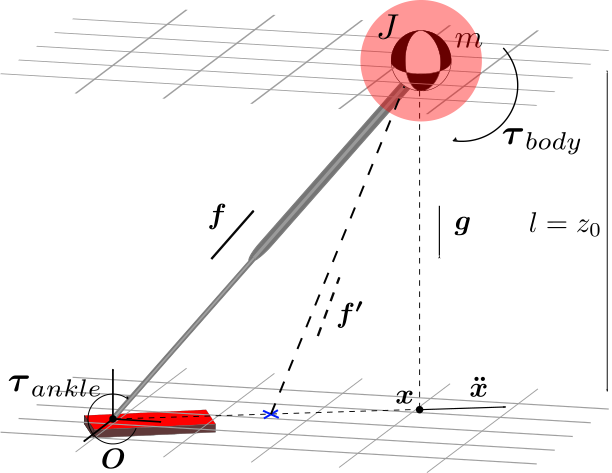
\includegraphics[width=0.5\textwidth]{STYLESTUFF/3DCoMwithfootinertia.png}
\caption{\ac{3D} motion of \ac{LIP} model with foot and body inertia. The blue cross points out the \ac{CMP} location.}
\label{fig:3dlipfootinertia}
\end{figure}

\subsection{Other Points}





% Energy of Walking
\section{Energy of Walking}
\subsection{LIP Orbital Energy} 
A crucial finding in an extended use of \ac{LIP} models can be found in \cite{kajita1992dynamic}. Because force is mass times acceleration: $F=ma$, impuse momentum is force times velocity: $I=Fv$ and the energy or work done by a force is the force times the distance, and thus the impulse integrated over the time interval: $E = Fs = \int Fv dt$, there can be reasoned that if one takes the time integral of the product of the second and the first derivative of a state, an expression for a normalized energy can be achieved: $\frac{E}{m}=\int av dt$. In the mentioned publication that same action is applied on Eq. \eqref{eq:LIPeom}:
\begin{equation}
\int (\ddot{x}-\frac{g}{l}x)\dot{x} dt = \frac{1}{2}\dot{x}^2-\frac{g}{2z_0}x +C=0
\label{eq:Elip}
\end{equation}
with $C$ the integration constant. The \ac{LIP} Orbital Energy is defined as $E_{LIP}=-C$. If $E_{LIP}>0$, the point mass will cross the $x$ position of the pendulum base with its current velocity. If $E_{LIP}<0$, the point mass will not cross the pendulum base and will have a turning point where the velocity becomes zero.

\subsubsection{The \acf{ICP}}
Although the finding of the \ac{LIP} Orbital Energy was very important for future robot motion modeling, more than a decade later \cite{pratt2006capture} introduced the \ac{CP}. Taking $E_{LIP}=0$ and taking the square root of Eq.  \eqref{eq:Elip} gives
\begin{equation}
x_{CP}=\sqrt{ \frac{z_0}{g}}\dot{x} 
\label{eq:cp}
\end{equation}
where $x_{CP}$ is the \ac{CP}, measured from the current pendulum tip position, based on the current tip velocity $\dot{x}$. This is the point where the velocity is exactly driven to zero and the pendulum is upright, where neither crossing of the pendulum base ocurred nor turning of body velocity. In \figref{fig:2dicp} a \ac{2D} visual explanation is given of this point.
\begin{figure}[h]
\centering
\includegraphics[width=0.4\textwidth]{STYLESTUFF/2DICP.png}
\caption{Visualization of path and states by the capture of the point mass according \ac{ICP} theory.}
\label{fig:2dicp}
\end{figure}
Later, the \ac{ICP} was introduced \cite{koolen2012capturability}, which gives a slightly different discription of the point:
\begin{equation}
x_{ICP}=x+\sqrt{ \frac{z_0}{g}}\dot{x} 
\label{eq:icp}
\end{equation}
where $x_{ICP}$ is the \ac{ICP}. In this way, the point can be described in the environment coordinates.
The $x$- and $y$-coordinate can be decoupled as in the equations of motion of Eq. \eqref{eq:LIPeom}. However, in the \ac{2D} horizontal plane, convergence to the capture point in one direction does not include convergence to the capture point in the other. In other words: the direction of motion is not restricted to move towards the pendulum base as in the sideview case.
\subsubsection{\ac{ICP} dynamics}
Because the ankle is not always located at the same location as the \ac{ICP} for the current horizontal velocity, for modeling and planning the time derivative is taken of the \ac{ICP}, which is named the \ac{ICP} dynamics \cite{koolen2012capturability}. This time derivative can be written as a function of the current \ac{ICP} location:
\begin{equation}
\boldsymbol{\dot{x}}_{ICP}=\sqrt{ \frac{g}{z_0}}\boldsymbol{x}_{ICP} 
\label{eq:cp}
\end{equation}
where $\boldsymbol{x}_{ICP}$ is the $xy$-vector of the \ac{ICP} location and assuming that the pendulum base is the origin.

\subsection{Nonlinear Orbital Energy}
Writing the nonlinear trajectory of a 2D model as $z=f(x)$, a similar expression of energy as \Elip  is derived in \cite{pratt2007derivation}
\begin{equation}
    E_{orbit}  = \frac{1}{2}\dot{x}^2\bar{f}^2(x)+gx^2f(x) - 3g\int_{x_0}^xf(\xi)\xi d\xi = \frac{1}{2}\dot{x}_0^2\bar{f}^2(x_0)+gx_0^2f(x_0).
\end{equation}
\Eorbit


\subsection{Boundedness Condition}
In \cite{lanari2014boundedness}:
\begin{equation}
x_u(t,z) = e^{\omega_0(t-t_0)}x_u(t_0) -\omega_0 \int_{t_0}^t e^{\omega_0(t-\tau)}r(\tau)d \tau
\end{equation}
bounded if:
\begin{equation}
x_u(t_0) = \omega_0 \int_{t_0}^{\infty} e^{-\omega_0(\tau-t_0)}r(\tau)d \tau
\end{equation}

This is extended in an varying height expression in...

% CoM Height Variation
\section{Related Works CoM Height Variation}
\subsection{Varying Height Terrain}
A lot of publications that incorporate the height variations in the terrain in the dynamic planning problem.
\cite{englsberger2013three} \cite{hopkins2014humanoid} and more..
\subsection{Mimic Natural Behavior}
Straight leg walking.
\cite{griffin2018straight} and more..
\subsection{Effects of Height Variation}
Research that investigates the energetic influences of height variations and impacts, often human orientated.
\cite{kuo2005energetic} \cite{lee1998determinants} \cite{gao2017increase} and more..
\subsection{Control for Balance}
Two publications that consider height variations as control input for balance:
\cite{koolen2016balance} \cite{caron2018capturability}
This is the focus in this thesis.

% Control Framework IHMC
\section{Humanoid Robotics at IHMC}
\subsection{Robots}
Atlas, Valkyrie.
\subsection{Walking States}
\begin{itemize}
	\item \ac{SS}
	\item \ac{DS}
	\item Toe-Off
\end{itemize}
\subsection{Planning}
\subsubsection{Footstep Planning}
User defined in \ac{GUI} or A* planner. Terrain information given by perception data (LiDAR).
\subsubsection{ICP Planning}
\ac{ICP} planning is the creation of a dynamical plan based on predefined footstep locations, the desired step time and the \ac{LIP} model of the system . Earlier approaches consider one \ac{CoP} knotpoint per footstep and integrate the \ac{ICP} dynamics backwards in time from the last footstep, considering the knotpoints to remain constant. Current improvements include double support, heel-toe multiple knotpoints, angular momentum prediction, continous \ac{CMP} trajectories instead of knotpoints.
\subsection{ICP Control}
From an \ac{CMP} and \ac{ICP} reference trajectory, the following control law is used to generate a desired \ac{CMP}:
\begin{equation}
    \mathbf{r}_{cmp,d}=\mathbf{r}_{cmp,r} + \mathbf{k}_{\xi}(\mathbf{\xi}-\mathbf{\xi}_r).
\end{equation}
From the desired \ac{CMP}, a desired horizontal linear momentum rate of change, a desired horizontal force, can be determined:
\begin{equation}
    \dot{\mathbf{l}}_{d,xy} = \frac{\mathbf{c}_{xy}-\mathbf{r}_{cmp,d}}{z_0}mg.
\end{equation}
The desired horizontal linear momentum rate of change $ \dot{\mathbf{l}}_{d,xy}$ is an input for the momentum-based controller.
\subsection{Momentum-based Control \& Inverse Dynamics}
\subsubsection{Dynamics humanoid}
\begin{itemize}

    \item End-effector motion:
$\bs{T}=\begin{bmatrix}\bs{\omega} \\ \bs{\upsilon} \end{bmatrix} = \bs{J}(\bs{q})\bs{\dot{q}}$, \quad Jacobian maps joint velocities to endeffector twist, or sometimes to other joint velocities.

    \item Centroidal momentum:
$\bs{h}=\begin{bmatrix}\bs{k} \\ \bs{l} \end{bmatrix} =\bs{A}(\bs{q})\bs{\dot{q}}$, \quad $\bs{A}=\bs{I}\bs{J}$ (Inertia * Jacobian)

    \item Dynamics:
$\bs{\dot{h}}=\begin{bmatrix}\bs{\dot{k}} \\ \bs{\dot{l}} \end{bmatrix} =\bs{A}\bs{\ddot{q}} +\bs{\dot{A}}\bs{\dot{q}} = \bs{W}_g + \sum_i\bs{W}_{gr,i} + \sum_i \bs{W}_{ext,i} $, \quad rate of change of centroidal momentum depends on external wrenches.

    \item Ground reaction wrench:
$\sum_i\bs{W}_{gr,i}=\bs{Q}\bs{\rho}$, \quad (contact matrix * basis vector multipliers). Wrench cone.
\end{itemize}

\subsubsection{Whole-body QP}
The desired vertical linear momentum rate is computed with the control loop
\begin{equation}
\bs{\dot{l}}_z =m(k_p(z-z_r) + k_d\dot{z}) 
\end{equation}
with bounds on resulting $\dot{z}$ and $\ddot{z}$.\\
QP: Find desired joint accelerations and ground reaction forces based on objectives. The objectives consist of a momentum objective, motion objectives, regularization terms and a null-space projection objective. The desired momentum is only determined by the desired linear momentum rate of change, the angular part is left unconstrained. An estimate of the amount of angular momentum rate of change that is needed to fulfill the desired linear momentum rate of change objective is given by the distance of the desired \ac{CMP} outside the foot polygon. If the \ac{CMP} is inside the foot polygon no angular momentum is needed, `ankle' strategies are enough to fulfill the desired linear momentum rate. Motion tasks include: desired foot trajectories, desired body orientation, desired spine joint position. Desired motion comes from PD-control. The null-space projection term can be used to input privileged joint accelerations, when the null-space of an robotic chain opens up, to avoid singularity.\\
The motion tasks and momentum tasks can conflict and the solution is always a trade-off, depending on the weights.
\begin{equation*}
\begin{array}{rlcl}
\displaystyle \min_{\bs{\ddot{q}}_d,\bs{\rho}} & \multicolumn{3}{l}{J_{\bs{\dot{h}}_d} + J_{\bs{J}} + J_{\bs{\rho}} + J_{\bs{\ddot{q}}_d}  + J_p} \\
\textrm{s.t.} & \bs{A}\bs{\ddot{q}}_d + \bs{\dot{A}}\bs{\dot{q}} = \bs{W}_g + \bs{Q}\bs{\rho}+\sum_i\bs{W}_{ext,i}\\
&\displaystyle \bs{\rho}_{min} \leq \bs{\rho}\\
&\bs{\ddot{q}}_{min} \leq \bs{\ddot{q}}_d \leq \bs{\ddot{q}}_{max}
\end{array}
\end{equation*}

\begin{equation*}
\begin{array}{rlcl}
$Momentum objective:$ & J_{\bs{\dot{h}}_d}= \bs{R}_{\bs{\dot{h}}_d}||(\bs{A}\bs{\ddot{q}}_d -\bs{b}||^2\\
$Motion objective:$ & J_{\bs{J}} = \bs{R}_{\bs{J}}||(\bs{J}\bs{\ddot{q}}_d-\bs{p})||^2\\
$Contact force cost:$ & J_{\bs{\rho}}=\bs{R}_{\bs{\rho}}||\bs{\rho}||^2 \\
$Joint acceleration cost:$ & J_{\bs{\ddot{q}}_d} = \bs{R}_{\bs{\ddot{q}}_d}||\bs{\ddot{q}}_d ||^2 \\
$Privileged configuration:$ & J_p = \bs{R}_p||(\bs{I} - \bs{J}_t^{\dagger}\bs{J}_t)\bs{\ddot{q}}_p - \bs{\ddot{q}}_d||^2
\end{array}
\end{equation*}

\begin{itemize}
\item $\bs{b} = \bs{\dot{h}}_d - \bs{\dot{A}}\bs{\dot{q}}$, \quad only linear momentum rate of change selected as objective: $\bs{S}\bs{\dot{h}}_d=\bs{\dot{l}}_d$
\item $\bs{p} = \bs{\dot{T}} - \bs{\dot{J}}\bs{\dot{q}}$, \quad (in case of end effector motion)
\item $\bs{J}= [\bs{J}_1^T\quad...\quad\bs{J}_N^T]^T$, \quad concatenated Jacobians of motion tasks
\item $\bs{J}_t = [(\bs{S}\bs{A})^T\quad \bs{J}^T]^T$, \quad big Jacobian for all tasks
\item $(\bs{I} - \bs{J}_t^{\dagger}\bs{J}_t)$,\quad null-space projector in case of a \textit{redundant} system (\textit{overdetermined}: joints have more degrees of freedom than end-effector motion)
\item $\bs{J}^{\dagger} = \bs{J}^T(\bs{J}\bs{J}^T +\mu^2)^{-1}$, \quad Moore-Penrose left (damped) pseudoinverse. $\mu>0$: damping factor. 

\end{itemize}

\subsubsection{Inverse Dynamics}
Desired joint torques $\bs{\tau}_d$ are calculated via inverse dynamics using solution of QP: $\bs{\ddot{q}}_d$ and $\bs{\rho}$.\\
\begin{itemize}
    \item  $\bs{\tau}_d = \bs{M}(\bs{q})\bs{\ddot{q}}_d + \bs{C}(\bs{q},\bs{\dot{q}}) + \bs{G}(\bs{q}) + \bs{J}^T \bs{f}$, \quad where $\bs{f}$ is the linear part of the ground reaction wrench.
\end{itemize}
